\documentclass[letter, 12pt]{article}
\usepackage[xdvi]{graphicx}
\usepackage{amssymb}
\usepackage{lineno}
\usepackage[lined,boxed,commentsnumbered]{algorithm2e}
\newcommand{\beq}{\begin{center}\begin{equation}}
\newcommand{\eeq}{\end{equation}\end{center}}
%\usepackage{setspace}
%\usepackage{pstricks,pst-node,pst-text}


\title{Efficient Batch LU Decomposition on GPU }
\begin{document}
\author{William J. Brouwer, Pierre-Yves Taunay\\ Research Computing and Cyberinfrastructure,\\ The Pennsylvania State University}

\maketitle


\abstract{There is much interest in porting algorithms to Graphics Processing Units (GPUs) suited to large matrices and vectors, indeed work on LU decomposition has been treated previously~\cite{lu}. This work revisits the LU decomposition procedure in the context of large numbers of small matrices (side $N$ less than 1024 elements), invaluable in several important applications. A GPU algorithm is presented alongside a CPU version of Crouts approach, demonstrating excellent scaling and timing characteristics.}

\section{Introduction}

Accelerating applications with Graphics Processing Units is stimulating ongoing interest in diverse fields within science and engineering. One attractive feature of the GPU platform lies in the natural scaling afforded by the architecture to increasingly large problems. For many algorithms, GPU performance relative to the CPU still remains high, despite recent hardware innovations in the latter. The oft-cited communication overhead derived from the separation of CPU and GPU devices, whether it be by bus or network  is rendered increasingly less relevant through good programming practice and hardware improvements.  Further, an increasing array of entry points to GPU acceleration are appearing in the form of libraries, explicit applications, languages as well as compiler directives in the form of OpenACC. Finally, GPU devices still deliver consistently more floating point operations per second per watt, of great relevance in the design and deployment of data centers in the quest for exascale computing. With regards to moving towards exascale, closely coupled with hardware innovations are algorithmic improvements that will permit users to leverage the resources efficiently. Numerical instability, poor scaling and performance are obviously detrimental to large problems. A very common task in science and engineering which may suffer from all the aforementioned drawbacks is the solution of linear equations; efficient and stable algorithms are much sought after. A growing number of applications break large domains into smaller ones, permitting the use of relatively expensive direct solvers based around (for example) LU decomposition~\cite{cbfm}, versus iterative solutions. LU decomposition also provides a viable method for the calculation of the matrix determinant; after execution of an in-place implementation, the determinant is available from the product of the diagonal elements. This is particularly useful in condensed matter physics, specifically in studies of the fractional quantum Hall effect based on construction of the Pfaffian wave function, which requires O(N!) determinant evaluations~\cite{sree}. The floating point operations per second performed in the LU algorithm for a small matrix obviously pales in comparison to those performed for a larger matrix, and justification for using GPU acceleration in this case is poor. However, where large batches of matrices are concerned or where the LU algorithm is one step in a larger workflow amenable to GPU acceleration, then the approach as detailed may be of great benefit. Towards porting both complete applications from the two different domains discussed previously to GPU, LU decomposition suited to the GPU architecture for large batches of small matrices was devised and tested against a CPU version. 
\section{Theory}   
As alluded to, the decomposition of matrix A into lower L (elements $\alpha_{ij}$) and upper U (elements $\beta_{ij}$) matrix :
\beq {\bf L.U} = {\bf A} \eeq
has the advantage of permitting the solution of linear systems in two steps, comprised of forward and backward substitution procedures, for multiple right hand sides in $Ax=y$. Crouts approach to LU decomposition solves the set of equations implicit to equation one; these are :
\beq \beta_{ij} = a_{ij} - \sum_{k=1}^{i-1} \alpha_{ik}\beta_{kj} \eeq
\beq \alpha_{ij} = \frac{1}{\beta_{jj}}\left( a_{ij} - \sum_{k=1}^{j-1} \alpha_{ik} \beta_{kj} \right ) \eeq
Numerical stability relies on suitable choice of pivot, or dividing element in the solution for $\alpha_{ij}$. Pivoting may be partial (a row interchange) or full (both row and column), the former is implemented in this work, commonly referred to as LUP decomposition. Following the approach detailed in Numerical Recipes~\cite{num}, the choice as to best pivot is made only after both equations 2 and 3 are solved for a given column, and thereafter the row swap and a scaling performed. Recording the row permutations in a separate vector is required for use with the solution of linear equations, in order that the right hand side vector be subsequently rearranged to suit. Equations 2 and 3 gives rise to $N^2 + N$ equations, whose overdetermined nature permits the setting of $N$ elements arbitrarily. A popular choice is to set the diagonal elements of $\alpha$ to one, followed in this work. Crouts approach to LU decomposition is summarized in algorithm 1.

\begin{algorithm}[t!]
\SetKwInOut{Input}{input}
\SetKwInOut{Output}{output}
\linesnumbered
\Input{$N\times N$ matrix $A$}
\Output{In-place LU decomposed matrix $A$}
\For{$i\leftarrow 0$ \KwTo $N-1$}{
	\For{$j\leftarrow 0$ \KwTo $N-1$}{
	find largest element $q$\;
	}
	$scale[i] = 1.0/q$\;
}
\For{$j\leftarrow 0$ \KwTo $N-1$}{
	\For{$i\leftarrow 0$ \KwTo $j-1$}{
		$sum = A[i][j]$\;

		\For{$k\leftarrow 0$ \KwTo $i-1$}{
			$sum -=A[i][k] * A[k][j]$\;
		}
		$A[i][j]=sum$\;
	}

	\For{$i\leftarrow j$ \KwTo $N-1$}{
		$sum = A[i][j]$\;

		\For{$k\leftarrow 0$ \KwTo $j-1$}{
			$sum -=A[i][k] * A[k][j]$\;
		}
		$A[i][j]=sum$\;
		find index $l$ of largest element $q=scale[i]$*fabs$(sum)$\;
	}

	\If{$j$ != $l$}{

	swap rows $j$ and $l$\;
	update $scale$ \;
	save permutation details \;  

	}

	 \If{$j != N-1$}{

		$sum = A[j][j]$ \;

		\For{$k \leftarrow j$ \KwTo $N-1$}{
			$A[i][j] /= sum$ \;
		}
	}
}

 \caption{LU decomposition with partial pivoting}
\end{algorithm}


\section{Implementation}


With the foreknowledge that the decomposition will be applied in batch, the mapping of computational thread to matrix is a seemingly reasonable strategy for a GPU implementation. However on the device this virtually eliminates the possibility of coalesced loads from global memory, and thread cooperation via shared memory, key requirements for good performance. At the other extreme, mapping thread to matrix element would introduce significant overhead in the form of synchronization, owing to dependencies between loops of algorithm 1. In a compromise between the two extremes, O(N) threads were assigned to the operations for each matrix, and individual CUDA thread block assigned one or more matrices to process. Referring to algorithm 1, there are at least two key points at which threads must cooperate. The first is the determination of scaling information, lines 1-6, which may be considered a separate scope to lines 7 forward. This task is readily solved using parallel reduction, a well known primitive.

Turning attention to the main steps of the algorithm, lines 8-14 perform updates to matrix elements above the diagonal, specifically column $j$. By assigning the index of the loop at line 8 to thread index, increasingly more threads in this scope work as the outer loop progresses; a brief summary of this scope as executed in CUDA is detailed in table 1. Within a warp, one may rely on SIMD execution, and thus ideally in this context, updated column elements are available when needed by threads with higher indices. As one might expect, matrices of side greater than a single warp require serialization of warp execution, due to the unpredictable way in which instructions are scheduled and dispatched within the Streaming Multiprocessor (SM), figure 1.


\begin{figure}[h!]   
\begin{centering}
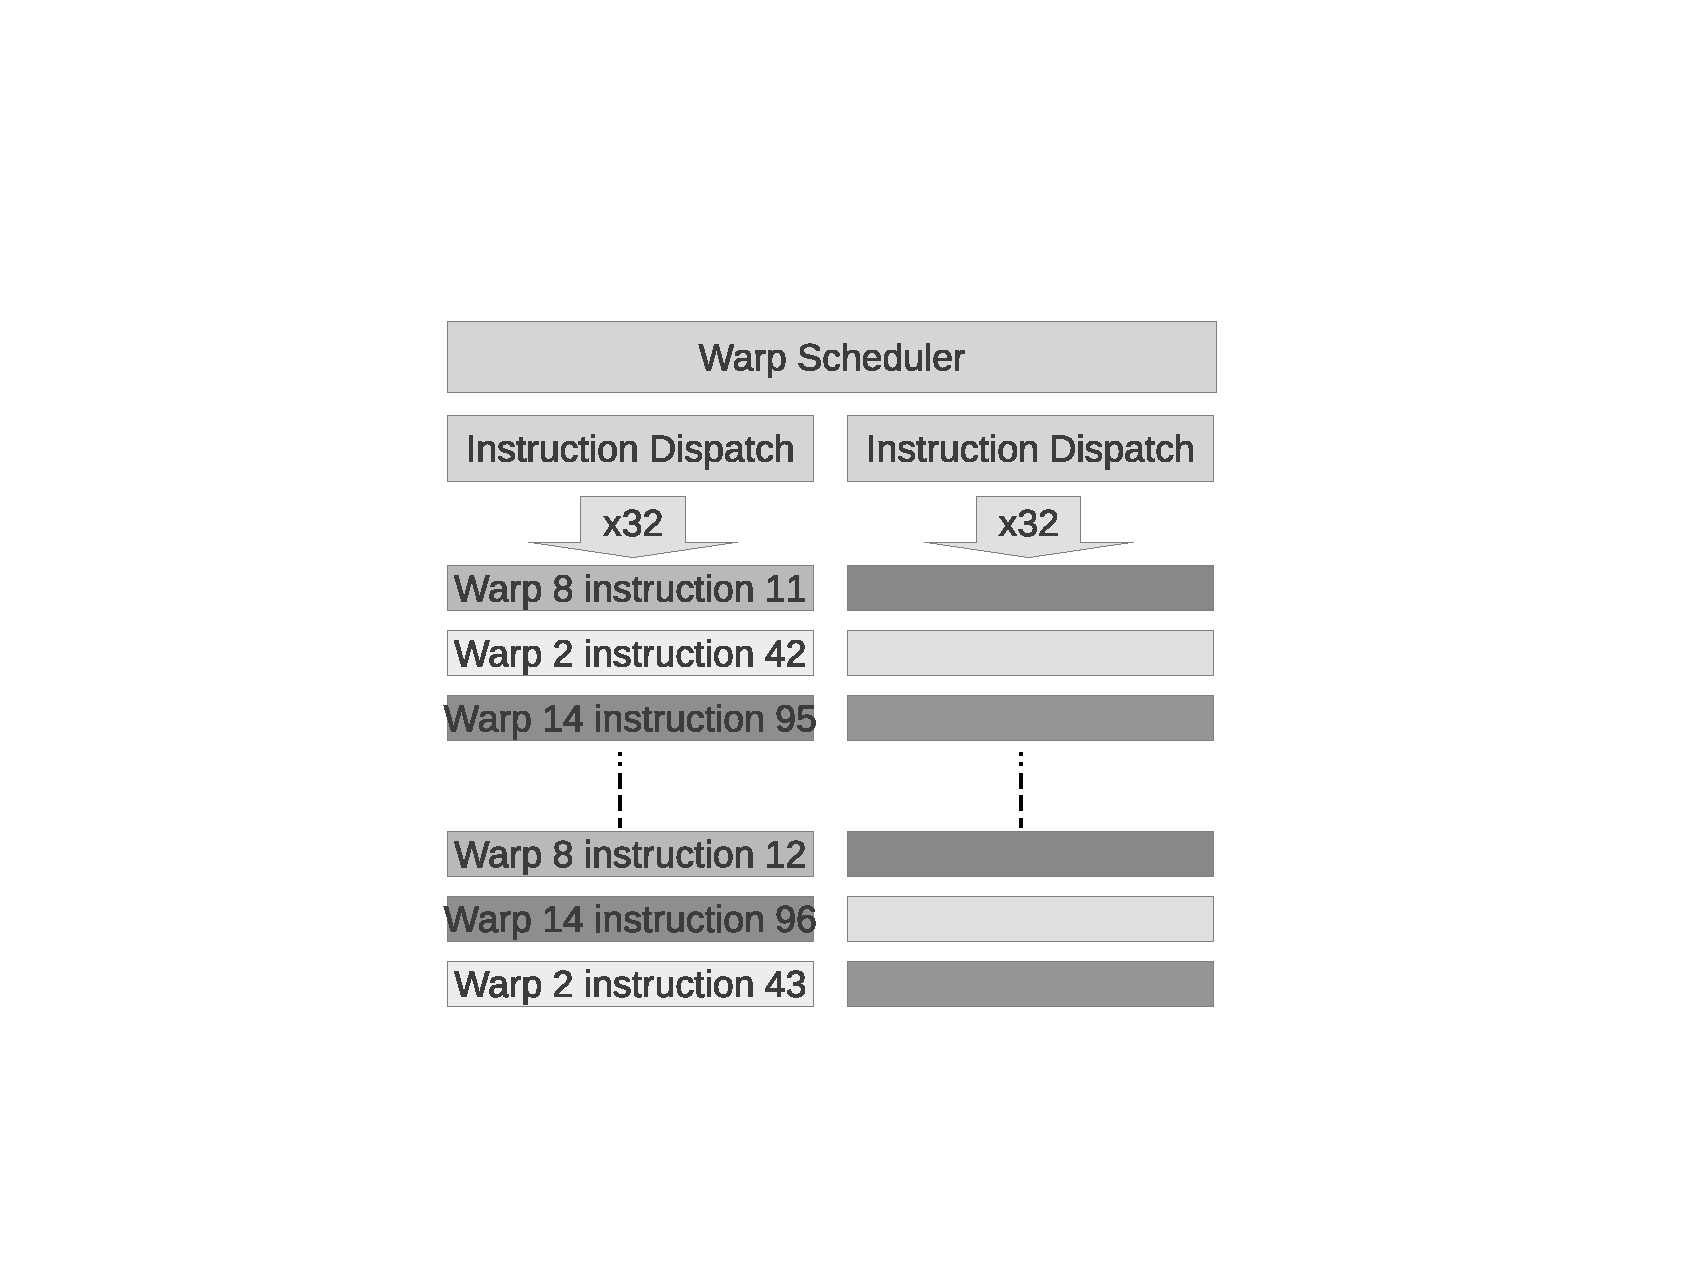
\includegraphics[width=0.9\textwidth]{kepler.eps} \caption{An example of instruction scheduling and execution in the Kepler streaming multi-processor} 
\end{centering}
\end{figure} 




No such limitations pervade lines 15-22, where loop index is also mapped to thread index, and column data is read from above the diagonal. Threads in this scope update from  diagonal downwards; however barrier synchronization is necessary before and after this scope. The particular column updated in a single iteration of the outer loop is cached in shared memory before line 8, and written bask to global after line 22. Shared memory buffers used for communication are declared using the volatile keyword, to ensure that write operations aren't optimized out during compilation. 


\begin{centering}
\begin{table}[h!]
\caption{Global memory read[], shared memory read(), write\{\}, critical$\dagger$ and arithmetic operations for several iterations and CUDA threads {\tt t\_id} of algorithm lines 7-14}
\begin{tabular}{llllll}
$k$ & t\_id 	& $j$=2 		& $j$=3 		& $j$=4 		& $j$=5 \\
\hline
- 	& 1	& (1,2)			& (1,3)			& (1,4) 		& (1,5) \\
0 	& 1 	& -[1,0]*(0,2) 		& -[1,0]*(0,3)		& -[1,0]*(0,4) 		& -[1,0]*(0,5) \\
-	& 1 	& \{1,2\} 		& \{1,3\}$\dagger$		& \{1,4\}$\dagger$ 		& \{1,5\}$\dagger$ \\
\hline
-	& 2	& 			& (2,3)			& (2,4) 		& (2,5) \\
0	& 2	&			& -[2,0]*(0,3)		& -[2,0]*(0,4) 		& -[2,0]*(0,5) \\
1	& 2 	&			& -[2,1]*(1,3)$\dagger$		& -[2,1]*(1,4)$\dagger$ 		& -[2,1]*(1,5)$\dagger$ \\
-	& 2 	&			& \{2,3\}		& \{2,4\}$\dagger$		& \{2,5\}$\dagger$ \\
\hline
-	& 3	&			&			& (3,4) 		& (3,5) \\
0	& 3	& 			& 			& -[3,0]*(0,4) 		& -[3,0]*(0,5) \\
1 	& 3	& 			& 			& -[3,1]*(1,4)$\dagger$ 		& -[3,1]*(1,5)$\dagger$ \\
2	& 3	& 			&			& -[3,2]*(2,4)$\dagger$ 		& -[3,2]*(2,5)$\dagger$ \\
-	& 3	& 			&			& \{3,4\} 		& \{3,5\}$\dagger$ \\
\hline
-	& 4	&			& 			& 			& (4,5) \\
0	& 4	&			&			&			& -[4,0]*(0,5) \\
1	& 4	&			&			&			& -[4,1]*(1,5)$\dagger$ \\
2	& 4	&			&			&			& -[4,2]*(2,5)$\dagger$ \\
3	& 4	&			&			&			& -[4,3]*(3,5)$\dagger$ \\
-	& 4	&			&			&			& \{4,5\} \\
\hline

\end{tabular}
\end{table}

\end{centering}


Once the column update is complete, and working threads have written elements $q$ in line 21 to another shared memory buffer, parallel reduction is employed in order to find the index of the pivot. Should the condition at line 23 be satisfied, then a row swap is completed by threads, storing temporary elements in registers. Thereafter, row elements are scaled by diagonal elements; once again loop index $k$ is mapped to thread. Barrier synchronization is employed before end of the outer loop at line 34. An abbreviated listing of the main CUDA kernel is recorded in the Appendix, based around the float2 type, for processing complex data.
\section{Results}
An implementation of Crouts algorithm was written in C for execution on CPU, for use with row-major storage format matrices and complex (single precision) floating point data. This routine was compiled using recent revisions of the Intel compiler, with flags {\tt -O3 -xHost} to ensure the highest degree of optimization, taking advantage of AVX hardware and instructions of the Sandy Bridge CPU. The main GPU kernel as described, driver code and supporting routines including parallel reduction were compiled using {\tt nvcc}, CUDA revision 5.0, initially with compute architecture 2.0, and optimization {\tt -O3}. Table 2 summarizes initial results, comparing execution times; profiling using {\tt nvvp} revealed a total global memory bandwidth of approximately 50 GB/s (38 GB/s read + 12 GB/s write). Both CPU and GPU routines were devoted to calculating the in-place LU decomposition alone, no permutations were stored, however the sign of the permutation was recorded in memory. The initial results were encouraging in that without tuning, the GPU routine was approximately a factor of 2-5 more performant than the CPU routine. Performance is degraded for a matrix of side 512, the cost of warp serialization adding significant overhead. The kernel does suffer the effects of un-coalesced loads of column data for processing. An attempt at optimization was developed to deal with this issue, operating on both the matrix and its transpose; this approach reduced execution time for a single kernel by as much as 20\%. While requiring approximately twice the global memory, the memory cost may be ameliorated through the use of streams, overlapping data-transfer and computation, not investigated in this work. The GPU kernel was further tested on the Kepler architecture, using a single K20m device. Several small changes were made; the thread block size was increased in several cases in order to take advantage of the higher thread throughput of the Kepler SM over Fermi (2048 versus 1536 threads)~\cite{kep}. The shared memory bank size was set in software to 8 bytes, increasing bandwidth slightly for processing the float2 buffers. The kernel was compiled for compute architecture 3.5 and optimization flag {\tt -O3}. Crouts algorithm when executed on the K20m device experienced a 1.3-2x performance improvement over the M2070 device, for minimal code and compilation changes. Most benefit was derived for the largest matrix and batch sizes, as anticipated.


\begin{centering}
\begin{table}[h!]
\caption{LU algorithm executed on M2070 and K20m GPU devices versus one Intel E5-2680 (Sandy Bridge) CPU thread}
\begin{tabular}{llllll}
Batch Size & Matrix Side &	M2070(s) & K20m (s) & CPU(s) & Matrices/Block \newline (M2070,K20m) \\
\hline
400 &	512 &	19.60 	& 	11.57 	&	39.30 	&	1,1 \\
800 &	256 &	2.40 	&	2.04 	&	8.47 	&	1,1 \\
1600 &	128 &	0.54 	&	0.49 	&	1.60 	&	1,1 \\
8000 &	64 &	0.37 	&	0.22 	&	0.94 	&	1,2 \\
16000 &	32 &	0.11 	&	0.08 	&	0.38 	&	2,4 \\
64000 &	16 &	0.06 	&	0.05 	&	0.31 	&	4,8 \\
\hline

\end{tabular}

\end{table}
\end{centering}

\section{Conclusion}

This work has detailed a new GPU approach to performing LU decomposition, for large batches of matrices of side less than 1024 elements. The kernel as outlined takes advantage of well known parallel primitives and displays highly favorable performance and scaling as compared to an equivalent CPU implementation. Performance for the basic kernel was improved significantly through introduction of several techniques guided by profiling. These techniques included configuring cache and shared memory in software, as well as optimizing thread blocksize, in order to take advantage of architectural advancements available in Kepler. 


\section*{Appendix}

\begingroup
\fontsize{6pt}{6pt}\selectfont
\begin{verbatim}
__global__ void luDecomposition ( float2 * inputMatrices, float * devSign ){

	// NOTES:
	// array indices have been simplified for readability
	// common tasks have been relegated to device functions	

        // temporary variables
        float2 sum,dum,tmp,tmpr,tmpl;

        // scratch space
        __shared__ float                sign [ NUM_MATRICES ];
        __shared__ volatile float       scale [ NUM_MATRICES * MATRIX_SIDE ];
        __shared__ volatile float2      reduce [ NUM_MATRICES * MATRIX_SIDE ];
        __shared__ volatile float2      vectors [ NUM_MATRICES * MATRIX_SIDE ];
        __shared__ volatile int         indices [ NUM_MATRICES * MATRIX_SIDE ];

        // index to matrix for processing
        int myMatrix    = threadIdx.x / MATRIX_SIDE;

        // index to vector for processing
        int vectorIndex = threadIdx.x % MATRIX_SIDE;

        // which warp 
        int myWarp      = vectorIndex / 32;


        // initialize permutation signs
        sign[threadIdx.x % NUM_MATRICES]=1.0f;

        // initialize shared memory
        initFloat2Buffer( vectors, FLOAT_MIN );


        // determine scaling information
        for (int i=0; i < MATRIX_SIDE; ++i){

                __syncthreads();

                // load shared memory

                vectors [ buf_index ].x = inputMatrices [ row_i_index ].x;
                vectors [ buf_index ].y = inputMatrices [ row_i_index ].y;

                __syncthreads();

                // find maxima by reduction
                findVectorMaxima ( vectors, vectorIndex, myMatrix );

                __syncthreads();
                // write scaling information
                if ( vectorIndex ==i ){

                        // should test for singular
                        scale [ scale_index ] = abs ( vectors [ buf_00 ].x );
                }
        }

        // initialize shared memory
        initFloat2Buffer ( vectors, 0.0f );

        for (int j=0; j<MATRIX_SIDE; j++){

                __syncthreads();

                // load the j column to shared
                vectors [ buf_index ].x         = inputMatrices [ col_j_index ].x;
                vectors [ buf_index ].y         = inputMatrices [ col_j_index ].y;

                __syncthreads();

                for (int i=0; i<WARPS_PER_MATRIX; i++){

                        __syncthreads();
                        if ( myWarp==i ){

                                if ( vectorIndex < j){
                                        sum.x = vectors [ buf_index ].x;
                                        sum.y = vectors [ buf_index ].y;

                                        for (int k=0; k< MATRIX_SIDE ; k++){

                                                if (k>=vectorIndex) break;

                                                tmpl = inputMatrices [ col_k_index ];

                                                tmpr.x = vectors [ buf_k ].x;
                                                tmpr.y = vectors [ buf_k ].y;

                                                sum.x -= (tmpl.x * tmpr.x - tmpl.y * tmpr.y);
                                                sum.y -= (tmpl.y * tmpr.x + tmpl.x * tmpr.y);

                                                vectors [ buf_index ].x = sum.x;
                                                vectors [ buf_index ].y = sum.y;

                                        }
                                }
                        }

                }

                __syncthreads();
                if ((vectorIndex >=j) && (vectorIndex < MATRIX_SIDE)){

                        sum.x = vectors [ buf_index ].x;
                        sum.y = vectors [ buf_index ].y;

                        for (int k=0; k< j; k++){

                                tmpl = inputMatrices [ col_k_index ];

                                tmpr.x = vectors [ buf_k ].x;
                                tmpr.y = vectors [ buf_k ].y;

                                sum.x -= (tmpl.x * tmpr.x - tmpl.y * tmpr.y);
                                sum.y -= (tmpl.y * tmpr.x + tmpl.x * tmpr.y);
                                vectors [ buf_index ].x= sum.x;
                                vectors [ buf_index ].y= sum.y;
                        }
                }
                __syncthreads();

                // write j column back to global
                inputMatrices [ col_j_index ].x = vectors [ buf_index ].x;
                inputMatrices [ col_j_index ].y = vectors [ buf_index ].y;

                // initialize shared memory
                initFloat2Buffer ( reduce, FLOAT_MIN );

                __syncthreads();

                if (vectorIndex >= j){

                        // init for pivot search by reduction
                        reduce [ buf_index - j ].x = abs ( vectors [ buf_index ].x ) /  scale [ scale_index ];
                        indices [ buf_index - j ]  = vectorIndex;
                }

                __syncthreads();
                findVectorMaximaKey ( reduce, indices, vectorIndex, myMatrix );
                __syncthreads();

                // possible row swap
                if (j != indices [ buf_00 ]){

                        int i = indices [ buf_00 ];

                        // each thread swaps one row element with another row element

                        sum                             = inputMatrices [ row_i_index ];
                        inputMatrices [ row_i_index ]   = inputMatrices [ row_j_index ];
                        inputMatrices [ row_j_index ]   = sum;

                        if (vectorIndex==0){
                                scale [ buf_i ]         = scale [ buf_j ];
                                sign [ myMatrix ]       *= -1.0f;
                        }
                }

                __syncthreads();

                // final scaling
                if ( j != MATRIX_SIDE-1){

                        dum = inputMatrices [ diag_j_index ];

                        if (vectorIndex >= j+1){

                                tmp                             = inputMatrices [ col_j_index ];
                                tmp                             = divide ( tmp, dum );
                                inputMatrices [ col_j_index ]   = tmp;
                        }
                }

                __syncthreads();

        }// end j loops

        // write out sign
        if (vectorIndex == 0) devSign [ sign_ind ] = sign [ myMatrix ] ;


}
\end{verbatim}
\endgroup
\begin{thebibliography}{30}
\bibitem{lu}
N. Galoppo, N. K. Govindaraju, M. Henson, D. Manocha, LU-GPU: Efficient Algorithms for Solving Dense Linear Systems on Graphics Hardware, 
in {\it ACM/IEEE conference on Supercomputing}, 2005
\bibitem{cbfm}E. Lucente, A. Monorchio, R. Mittra, An Iteration-Free MoM Approach Based on Excitation Independent Characteristic Basis Functions for Solving Large Multiscale Electromagnetic Scattering Problems, {\it IEEE Transactions on Antennas and Propagation} , 56(4):999--1007, 2008
\bibitem{sree} G. J. Sreejith, S. Jolad, D. Sen, J. K. Jain, Microscopic study of the $\frac{2}{5}$ fractional quantum Hall edge, {\it Phys. Rev. B}, 84(24):245104,2011
\bibitem{num} W. H. Press, B. P. Flannery, S. A. Teukolsky, W. T. Vetterling, Numerical Recipes in C, The Art of Scientific Computing, CUP, 2nd Ed., 1993
\bibitem{kep} http://www.nvidia.com/content/PDF/kepler/NVIDIA-Kepler-GK110-Architecture-Whitepaper.pdf

\end{thebibliography}

\end{document}
